\newpage

\section{Metode og Proces}
I nedstående afsnit fremlægges metoder og processer brugt til udviklingen af
Dungeons and Gnoblins spillet.

\subsubsection{Gruppedannelse}
Gruppen blev dannet på baggrund af at vi som studerende selv skulle finde medlemmer og danne projektgrupper. 4 af gruppens medlemmer var dannet inden semesterets start og de resterende 4 blev indmeldt efter offentliggørelsen af semesterprojektet. Gruppen redegjorde først ideer til projektet og blev hurtigt forventningsafstemt om projektets resultat skulle være middelmådigt. 

\subsubsection{Projektforløb og møder}
Projektets endelige mål har været implementeringen af et text-based adventure game.
Hertil har gruppen gjort brug af agile processen til at imødekomme dette mål.

Først har gruppen specifiseret Kravspecifikationerne for spillet, med ønsker om
hvilke features spillet har skulle inkludere. Continuous integration er dernæst
været et vigtigt værktøj til implementeringen af de ønskede features, med et klart
ønske om at integrere nye features ind i projektet få tidligt som muligt.\\

I løbet af projektforløbet blev der afholdt to faste ugentlige møder. Et internt gruppemøde om mandagen og vejledermøde om onsdagen. Hertil var der fra start uddelt rollerne Mødeleder og referent til gruppens medlemmer som gik på skift hver uge. Til hvert møde blev der gennemgået hvad der var blev arbejdet med, hvilke udfordringer der forekom samt hvad der fremadrettet skulle arbejdes med for hver af gruppens medlemmer. Dette gjorde vi i form af SCRUM for at give et bedre overblik for projektets fremgang og dermed vurderer om gruppen var bagud eller foran ift. Gruppens tidsplan. Vores SCRUM-proces var ikke avanceret hvor der blev koordineret SCRUM Master og Product Owner, men blev derimod anvendt som redskab til at skabe et overblik over arbejdsfordelingen og udviklingen. Tidsplanen blev udarbejdet ved projektets start og havde formålet at give gruppen deadlines for projektets udviklingsproces.

\begin{figure}[H]
  \centering
  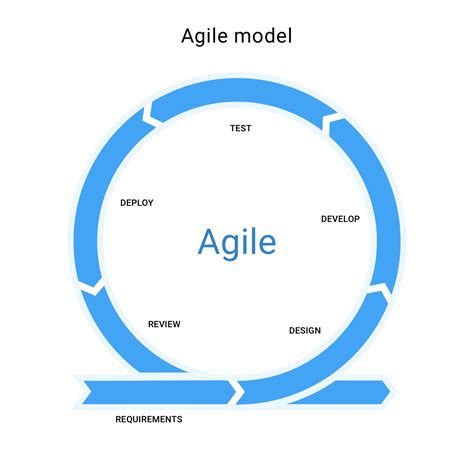
\includegraphics[scale=.5]{02-Body/Images/Agile.png}
  \caption{Viser et billed af agile modellen som består af mangle iterationer
           af design, develop, test, og deploy. Dette minder om continuous integration
           og har hindret mange problemmer for udviklingsforløbet}
  \label{fig:Agile}
\end{figure}

SCRUM og AGILE bringer klarhed til medlemmerne om deres roller og opgaver over en 
kommende tidperiode med en backlog over opgaver, som skal færdiggøres over et sprint (1 uge).
Ugentlige opdateringer og møder omkring potentielle problemmer udviklingsforløbet betyder
at gruppen har kunne tage hånd om evt. problemmer tidligt i forløbet og derved løse dem
før de har udviklet sig til større problemmer.

Til styring og implementering af souce code har vi benytte git som et version control system.
fordelen ved git er at det tillade flere udviklere at arbejde på det samme projekt og integere 
deres løsninger. Der er dog chancer for merge konflikter hvilket kan, i værkste tilfælde, før
til problemmer med at integrer de forskellige løsninger korrekt med hinanden.

\subsection{Modellering}
Projektet benytter UML til at beskrive og modellere software-- arkitektur
og design, hvilket gør det nemt at simplificere og visualisere strukturen på software
løsningen. 

Selve arkitekturen er vist med C4 modellen som giver et lageret indblik i både
akitekturen på et højt niveau, men med evnen til at give en detaljeret beskrivelse
af systemmets komponenter og deres kommunikation med hinanden.

\begin{figure}[H]
  \centering
  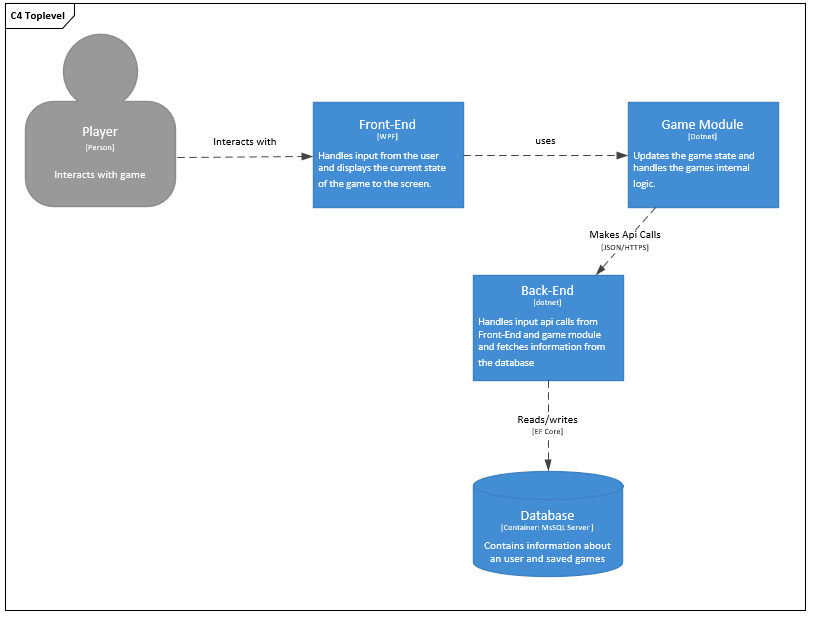
\includegraphics[scale=0.8]{02-Body/Images/C4TopLvlDB.PNG}
  \caption{}
  \label{fig:c4}
\end{figure}

STM og SD diagrammer er brugt til at give programmets udførsel struktur, og fungere
som en hjælp til at visualisere programmets forskellige states og flow of execution.
Det giver et nemt overblik over hvordan funktionskald mellem forskellige komponenter
har skal fungere således, at der ikke opstår misforsåelse grupperne imellem. 

Generelt er arkitekturen opbygget som "pseudo" diagrammer. Dvs. de ligner ikke fuldstændigt 
det endelige design, men har til formål at vise den overordnede tankegang i systemet og 
samtidig virke som et udviklingsværktøj til at videreudvikle systemet. Da der i gruppen 
er blevet arbejdet iterativt, er der forskelle mellem diagrammer for arkitektur og design,
da der er blevet tilføjet flere moduler og funktioner undervejs. Den overordnede tanke i 
projektet er der dog ikke blevet ændret på.

\subsubsection{Iterativ Udviklingsforløb}

AGILE og continuous integration fungere på en naturlig iterativ måde, der tillader 
ændringer til måde designet og implementeringen undervejs i udviklingsforløbet.
Under hvert SCRUM møde er der taget stilling til om, der skulle laves ændringer i 
gruppens tilgang til projektet, altså om en implementering skulle ændres. \\

Et eksempel har været kommunikationen mellem Game Engine og Frontend, hvor frontend
har haft svært ved at håndtere komplicered return types. Der er sålede lavet
ændringer for at gøre det nemmere for frontend at udnytte den infomation som Game Engine
har returneret efter et funktionskald.

Denne flexible arbejdsmetode har igen ført til at problemmer ikke har kunne vokse men
at der blevet taget hånd om dem mens det stadig har været muligt at håndtere dem.

